%%% Thesis chapter1 --------------------------------------------------
\chapter{Role of Nuclear Quantum Fluctuations
on an electrochemical interface: the case of Pt(111) and water } \label{chapter3}
%\footnotetext{Reprinted (adapted) with permission from \emph{Surface Science}, \textbf{2016}, 644, 69-79.}
\ifpdf
    \graphicspath{{Chapter3/Chapter3Figs/}}
\fi
 
% ------------------------------------------------------------------------
\section{Introduction}

Electrochemical reactions play an important role in the inter-conversion of electrical and chemical energy with applications in batteries\cite{etacheri2011challenges}, fuel cells\cite{felseghi2019hydrogen}, water splitting devices\cite{grigoriev2020current}, etc. Some of the important aqueous electrochemical reactions include N$_2$ reduction\cite{qing2020recent}, CO$_2$ reduction reaction\cite{lim2014review}  (CO$_2$-RR), H$_2$O$_2$ synthesis\cite{jiang2018selective}, hydrogen evolution/oxidation reaction\cite{zeng2015recent,strmcnik2013improving} (HER/HOR) and oxygen evolution/oxidation reaction\cite{suen2017electrocatalysis,stacy2017recent} (OER/ORR). These electrochemical processes usually occur at the interface between a solid electrode immersed in an aqueous electrolyte. As a result, it is necessary to investigate the microscopic interfacial structure and understand its correlation with the macroscopic properties. The most important electrochemical property is the electrode potential which is measured as a half cell redox reaction against the standard hydrogen electrode (SHE). Experimental data from Trasatti\cite{trasatti1991structure,trasatti1983structuring} show that the electrode potential is related to the work function of the water covered electrodes which are mostly metals and their derivatives\cite{conway2002interfacial,subbaraman2011enhancing,le2009hydrogenases,du2012catalysts,jaramillo2007identification,voiry2013enhanced,merki2011recent}. The interfacial structures affect this work function and indirectly modify the electrode potential. Li et al.\cite{li2021establishment} report that the work function of the metal is affected by the interfacial dipoles originating from charge reorganization and preferential orientation of the polar (O-H) bonds in the water layer.

Thus, in this work, we study the electrochemical aqueous interface of the commercially important Pt electrocatalysts. The resulting Pt/water interface is used widely in various electrochemical processes such as HOR/HER\cite{eftekhari2017electrocatalysts} and OER/ORR\cite{sui2017comprehensive} due to its high activity and performance. Over the years, surface experiments such as atomic force microscopy\cite{tian2022visualizing}, Scanning Tunneling Microscopy\cite{carrasco2012molecular} (STM), and others\cite{magnussen2019toward} have looked into the molecular structures at these interfaces. Much recently, Tian et al.\cite{tian2022visualizing} using an improved qPlus based AFM technique has been able to directly visualize Zundel and Eigen cations at 5 K under ultra vacuum conditions. Since these microscopic techniques operate at extreme conditions, only a qualitative picture of the interface is described. The accurate description of the actual electrochemical interface is difficult for both experiments and theoretical methods. Nevertheless, many theoretical studies have been undertaken to elucidate the molecular structure using first principle studies\cite{karlberg2007cyclic,karlberg2007cyclic,skulason2007density} along with molecular dynamics (MD) calculations\cite{li2021establishment,sakong2018electric,le2018structure,lan2020ionization} in order to sample the thermal fluctuations. For example, Lan et al.\cite{lan2020ionization} and Li et al.\cite{li2021establishment} using \textit{ab initio} MD report that the interfacial water forms a bilayer where some water molecules are chemisorbed on the Pt surface. Additionally, Le et al.\cite{le2018structure} shows the formation of bilayer can be tuned by introducing an external electric field. On the contrary, in the absence of an external electric field, Sakong et al.\cite{sakong2018electric} could not observe the formation of bilayer. The use of different dispersion effects explains this disagreement\cite{gross2022ab}.
%revised PBE-D3 exchange-correlation functional\cite{hammer1999improved,grimme2010consistent}, in contrast to the PBE-D3 functional\cite{GGA-PBE1996,grimme2010consistent} used in the above studies. 
However, all these studies, in agreement with each other, find that the water layer donates its electronic charge to the surface Pt atoms. Le et al.\cite{le2018structure} and Li et al.\cite{li2021establishment} report that the electronic rearrangement creates an interfacial dipole that reduces the work function of the water covered Pt by 1.07 and 1.1 eV respectively. Overall, these reports do not mention the formation of Zundel/Eigen cations observed using the qPlus-AFM\cite{tian2022visualizing} probe. 

Since water constitutes of the light hydrogen nuclei, the modelling of the Pt/water interface was improved by incorporating the quantum effects of the nuclei. Litman et al.\cite{litman2018decisive} using Path integral molecular dynamics (PIMD) found that the NQEs increase the dissociation probability of water molecules in water wires on stepped Pt(221) surface which leads to 0.04 eV decrease in the work function of the Pt(221) surface. In the case of Pt(111)/water interface, Lan et al.\cite{lan2020ionization} reports that NQEs help the chemisorbed water to dissociate into hydroxyl ion and proton where the former is chemisorbed over the Pt surface and the latter gets solvated into the water layer. Thus, the incorporation of NQE is essential in describing the interface structure obtained from experiments\cite{tian2022visualizing,magnussen2019toward}. However, these \textit{ab initio} PIMD simulations are computationally very expensive and is rarely used. Therefore, in this study, we switched to the quantum mechanics molecular mechanics (QMMM) based PIMD simulations. This method treats the Pt metal and the interface water at the quantum mechanical level whereas the bulk region is treated using classical force fields. This allows a cheaper assessment of the potential energy surface without losing the quantum mechanical information of the interface. The details regarding the QMMM setup and the QMMM $+$ PIMD is explained in the methods section. 

The clean Pt(111)/water interfaces as discussed above are available for a very narrow range of electro-chemical conditions\cite{gross2022ab} and are usually covered with electrolytic species\cite{gross2022ab} such as OH$^-$, SO$_4^{2-}$, CO, H and others depending on the type of solution and the electrochemical conditions. Amongst the different species, adsorbed hydrogen atoms form a crucial intermediate in the Volmer step (equation \ref{volmer}) of the HOR/HER process.
\begin{equation}
    \label{volmer}
    H_{ads} \rightleftharpoons H^+(aq) + e^-
\end{equation}
Since, the adsorption energy of the hydrogen has been reported as a descriptor in the activity of the HER/HOR processes, many theoretical studies\cite{kristoffersen2018oh,kronberg2020coupling,le2021modeling,sakong2018electric} have modelled the hydrogen covered Pt(111)/water interface and investigated the role of coverage. These studies report that the adsorbed hydrogen atoms compete with the water chemisorption and displaces the chemisorbed water. Kristoffersen et al.\cite{kristoffersen2018oh} (for H coverage $>$ 0.33 ML) and Sakong et al.\cite{sakong2018electric} (for 1 ML H coverage) report that the adsorbed hydrogen desorb from the Pt surface into the aqueous layer thereby decreasing the pH of the interface layer. On the contrary, Kronberg et al.\cite{kronberg2020coupling} did not find any hydrogen desorption. Similar observations are also reported by Le et al.\cite{le2021modeling} for a hydrogen coverage of 0.66 ML on the electrified Pt/water surface. The various contradictions prompted us to investigate the hydrogen covered Pt(111)/water interface at an intermediate coverage of 0.5 ML. %0.66 ML\cite{le2021modeling,ford2005atomic} using QMMM simulations.
In spite of our extensive literature survey, we found limited reports\cite{lan2022nuclear,fang2017simultaneous,lan2020ionization,litman2018decisive} investigating the NQEs at these interfaces where most of them are either concerned with few water molecules\cite{litman2018decisive} or a layer of structured water/ice\cite{yan2020nuclear}. Thus, we performed QMMM and QMMM $+$ PIMD simulations to investigate the role of NQEs at the clean and 0.5 ML H covered Pt(111)/water interface. Our study finds that NQEs dissociate the chemisorbed water at the clean interface where the dissociated hydroxyl is adsorbed on the surface and the dissociated proton gets solvated into the water layer. The solvated proton propagates throughout the liquid layer predominantly in the Zundel form. In the case of hydrogen covered Pt/water interface, irrespective of whether the NQEs are incorporated or not, we observe some of the adsorbed hydrogen atom to desorb and enter the water layer as solvated protons. The microscopic structure at the interface creates an interfacial dipole that affects the work function of the water covered metal. The interfacial dipole originates because of two effects: charge reorganization at the interface and preferential orientation of the polar O-H polar bonds. The work function change due to the charge reorganization (OH orientational) dipole decreases (increases) the work function. However, OH orientational dipole is quite small compared to the charge reorganization dipole. Hence, the net effect is that NQEs tend to decrease the total work function thereby making the electron abstraction from both the clean and H covered Pt/water interface easier. 

The overall chapter is arranged in the following manner: Section \ref{methodd} describes the QMMM setup, the implementation of the coupling of QMMM $+$ PIGLET and the computational details. Section \ref{resultss} contains the results and discussion regarding the role of NQEs at the clean and H covered electrochemical Pt/water interface. Finally, the last section concludes the entire study. 

\section{Methodologies}
\label{methodd}

\subsection{Models of the interface} 
The Pt/water interface is modelled by constructing a surface from 
bulk platinum and wetting it with layers of water molecules. In this study, we have investigated the most stable (111) surface, which is modelled using a four layer slab. Each of these Pt layers has two atoms inside an orthorhombic (1 $\times$ 1) surface unit cell of dimensions 2.77 \AA~$\times$ 4.80 \AA. Experimental values\cite{habershon2009competing} of pair correlation functions (g$_{OO}$, g$_{OH}$ and g$_{HH}$) for the bulk water reveal a local structuring that expands to $\sim$6 \AA{}. Therefore, a minimum cell dimension of 12 \AA{} is needed to capture the local structuring in liquid water. This requirement is ensured by depositing water layers over a (7 $\times$ 4) supercell of the Pt surface. As a result, each of the Pt layers contains 56 atoms. 480 water molecules were used to model the liquid water resulting in a thickness of about 35 \AA{}. Since the calculations have been performed using periodic boundary conditions, we have added an additional 25 \AA{} of vacuum to minimize the spurious interactions between the periodic images along the direction normal to the Pt surface. Figure \ref{fig:Slide6}(a) shows a representative snapshot of the Pt(111)/water system. 


\begin{figure}
    \centering
    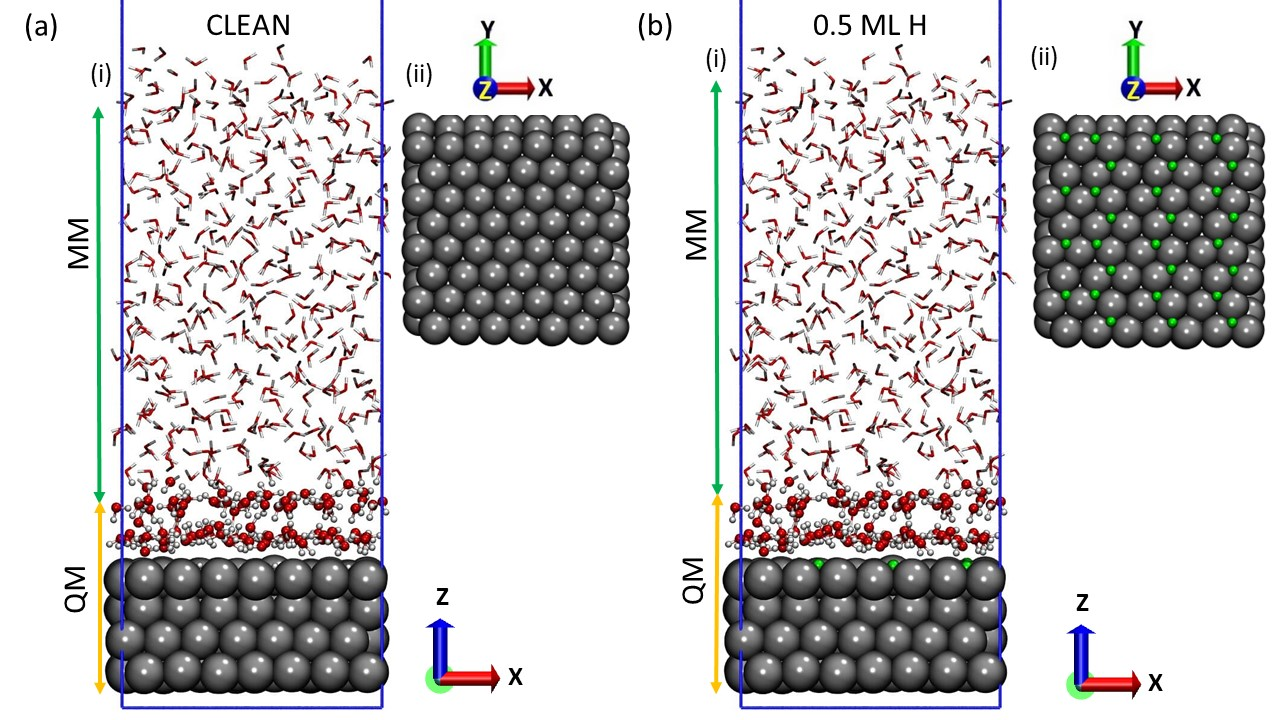
\includegraphics[width=15cm ]{./Chapter3/figures/Slide6.jpg}
    \caption{A random snapshot of the (a) clean and (b) 0.5 ML H Pt(111)/water systems. (i) The side view showing the QM and MM subsystems of the QMMM setup. (ii) The top view of the Pt surface along with chemisorbed hydrogen (for 0.5 ML H system which are shown as green balls) on the ``fcc" site of the Pt surface. }
    \label{fig:Slide6}
\end{figure}

For the hydrogenated interface half a monolayer (ML) of hydrogen atoms were randomly deposited at the face centered cubic (fcc) sites of the Pt(111) surface in contact with the water layer. The choice of fcc site is in accordance with previous DFT-based static calculations\cite{kronberg2020coupling,yan2018hydrogen}, and \textit{ab initio} MD\cite{kronberg2020coupling} and PIMD simulations\cite{yan2020nuclear}, which report that the H atoms prefer to occupy the ``fcc" sites. Figure \ref{fig:Slide6}(b) is a representative snapshot of the Pt(111)-0.5 ML H/water system. 

\subsection{Implementation of Coupling of QMMM and PIMD in CP2K}

As mentioned in Chapter \ref{theoreticalmethods} of the thesis, in order to capture the effects of
the quantum fluctuations of the nuclei one needs to perform path integral molecular
dynamics simulations where the total energy of several replicas of the system
needs to be computed. For the Pt/water interface studied here, 
bond breaking and bond formation processes are known to occur, thereby necessitating
an accurate description of the potential energy surface (PES), which
can be achieved using a quantum mechanical treatment of the whole system.
Usually the potential energy surface on which the system evolves in the MD
simulations can be obtained, within reasonable accuracy, from DFT based calculations.
However, due to the absence of long range order in the liquid part of the interface,
there are a large number of atoms and electrons, thereby making a full \textit{ab 
initio} description, even at the level of DFT, of a single replica
of the complete Pt/water system, computationally prohibitive. Hence, we have adopted the 
cheaper alternative of computing the PES from Quantum Mechanics Molecular Mechanics 
(QMMM) based method in which a part of the system is treated quantum mechanically
while the remaining is treated classically.

\begin{figure}
    \centering
    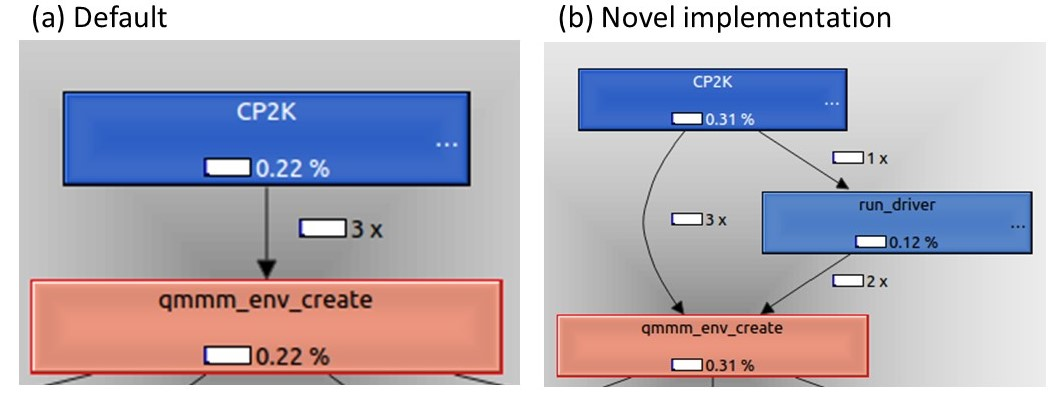
\includegraphics[width=15cm ]{./Chapter3/figures/Slide7.jpg}
    \caption{The callgraph for the ``qmmm\textunderscore env\textunderscore create" subroutine in the CP2K package generated from QMMM $+$ PIGLET simulation in (a) the default and (c) our novel implementation.}
    \label{fig:Slide7}
\end{figure}

As described later, we have used the CP2K software which computes the QMMM
energies along with the i-PI package\cite{kapil2019pi}, the latter is the driver
for the PIMD simulation. During the dynamics, there is exchange of atoms
between the QM and MM regions. This dynamic exchange of atoms are handled
by the ``qmmm\textunderscore env\textunderscore create" subroutine in CP2K.
However, in the existing implementation of QMMM $+$ PIGLET simulation, the ``run\textunderscore driver", a module for i-PI that controls the dynamics does not
call the above mentioned subroutine as shown in the callgraph
in Figure \ref{fig:Slide7}(a). As a result the number of atoms in the QM and MM
regions erroneously remain constant. To solve this we modified
the code to ensure that the module ``run\textunderscore driver" calls the 
``qmmm\textunderscore env\textunderscore create" subroutine as shown in the
callgraph in Figure \ref{fig:Slide7}(b).


Ensuring dynamic exchange of atoms between the QM and the MM regions gave rise to
another problem. The number of QM and MM atoms in different beads became unequal
which resulted in the mixing of MM and QM forces for the same atom. In order to maintain the same number of QM and MM atoms in each bead, we have used the
centroid of the ring polymer to segregate the QM and MM atoms in all the 
beads/replicas.  

\subsection{Computational details}
In our QMMM MD setup, the MM subsystem contains water molecules in the bulk region of the liquid water whereas the QM subsystem includes the Pt atoms and all the water 
molecules that lie within a distance of 7 \AA~from the surface Pt atoms at the
interface.
The liquid water is dynamic as the 
water molecules exchange between the interface and the bulk region of the 
liquid\cite{sakong2020water}. Our QMMM setup ensures this dynamic exchange by 
switching the identity of a MM (QM) water molecule to a QM (MM) molecule on entering 
(exiting) the boundary between the QM and MM subsystems. The identity switch is based 
on the relative distance of the water molecules from the Pt surface, which in
our case is 7 \AA, and is commonly 
known as the adaptive QMMM\cite{bernstein2012qm}. The interaction between the atoms in the MM and QM regions are modelled using the electrostatic embedding scheme\cite{laino2006efficient}. More details regarding the setup can be found in our previous work\cite{hardikar2019theoretical}.

All the quantum mechanical calculations are performed using the Quickstep\cite{kuhne2020cp2k} module of the CP2K package. The Quickstep module is based on the Gaussian and Plane wave (GPW) based implementation of the density functional theory (DFT) where the electronic exchange and correlation effects are approximated using the generalized gradient approximation (GGA) based parameterization proposed by Perdew, Burke and Ernzerhof\cite{GGA-PBE1996}(PBE). Additionally, van der Waals interactions are also included through Grimme's D3 dispersion correction\cite{grimme2010consistent}. The electron-ion interactions are described by the Goedecker, Teter, and Hutter\cite{goedecker1996separable} (GTH) pseudopotentials. Double-zeta valence polarisation (DZVP) basis set is used.
The charge density is expanded on a grid with a plane wave cutoff of 300 Ry. The calculations are performed at the $\Gamma$-point only. On the other hand, modified (flexible) SPC/E parameters are used to calculate the forces on the MM subsystem. The benchmarks and validations of the force field parameters are reported in the supporting information of our previous work\cite{hardikar2019theoretical}. 

Since this study investigates the manifestations of NQE at the Pt/water interface, the quantum partition function of the atomic nuclei needs to be sampled. Hence, we have
performed path integral molecular dynamics simulation (coupled to the coloured noise generalized Langevin equation based thermostat, PIGLET\cite{ceriotti2012efficient}) where the QMMM is used to compute the potential energy surface (QMMM $+$ PIGLET). The dynamics (PIGLET simulation) is handled by the i-PI package\cite{kapil2019pi} and the CP2K package provides the i-PI with energy and atomic forces. 

All the MD simulations have been performed at 298 K. The results of the QMMM 
simulations for the clean and 0.5 ML H systems are obtained from their respective 10 ps 
of equilibrated trajectories. A random snapshot from the equilibrated QMMM 
trajectory is then used
as an initial configuration to run the QMMM $+$ PIGLET simulation. Each of the two 
QMMM $+$ PIGLET simulations for the two systems contains 9 ps of equilibrated data. 
All the four simulations (two QMMM and two QMMM $+$ PIGLET) has a time step of 1 fs 
for integrating the equations of motion. Based on the convergence studies performed by Ceriotti and 
Manolopoulos\cite{ceriotti2012efficient} on liquid water, six beads are used for the
QMMM $+$ PIGLET simulations.

In order to validate the QMMM $+$PIGLET coupling, we performed QMMM $+$ PIGLET and
Born-Oppenheimer $+$ PIGLET simulation for the clean system (with a smaller size) and
compared their results in Appendix \ref{appendix5}. We find that at the interface, 
the results obtained from both the simulations are similar, thereby giving
confidence that our new implementation is working fine.


\section{Results}
\label{resultss}
    

\subsection{Effect of NQEs on the structural properties of the interfaces}
\label{clean-yes}

In this section we describe how NQEs affect the structural properties
of the Pt(111)/water and Pt(111)-0.5ML H/water interfaces. The distance between the Pt slab and the interface water layer provides a measure of the interaction between the solid and the liquid. Moreover, as one moves from bulk water to the interface, the abrupt termination of the water layer results in a static inhomogeneity that might affect the
structural properties of the interface. In order to quantify these
we have computed the planar average of the density of water molecules as 
a function of the distance from the Pt surface using the following equation:

\begin{equation}
    \label{densitt}
    \rho_{density}(z) =(l_xl_y\Delta z)^{-1} (\, p_O (z) \, m_O + p_H (z) \,m_H \,)
\end{equation}

where $\rho_{density}(z)$ is the water density at z, $l_x$ and $l_y$ are the box lengths and $\Delta z$ is the bin size along the z direction. $m_O$ and $m_H$ indicates the mass of oxygen and hydrogen atoms respectively. $p_O (z)$ and  $p_H (z)$ are the normalized probability distributions of the number of oxygen and hydrogen atoms between $z$ and $z+\Delta z$. The density in our case is calculated by using a bin size of 0.05 \AA.

\begin{figure}
   \begin{center}
    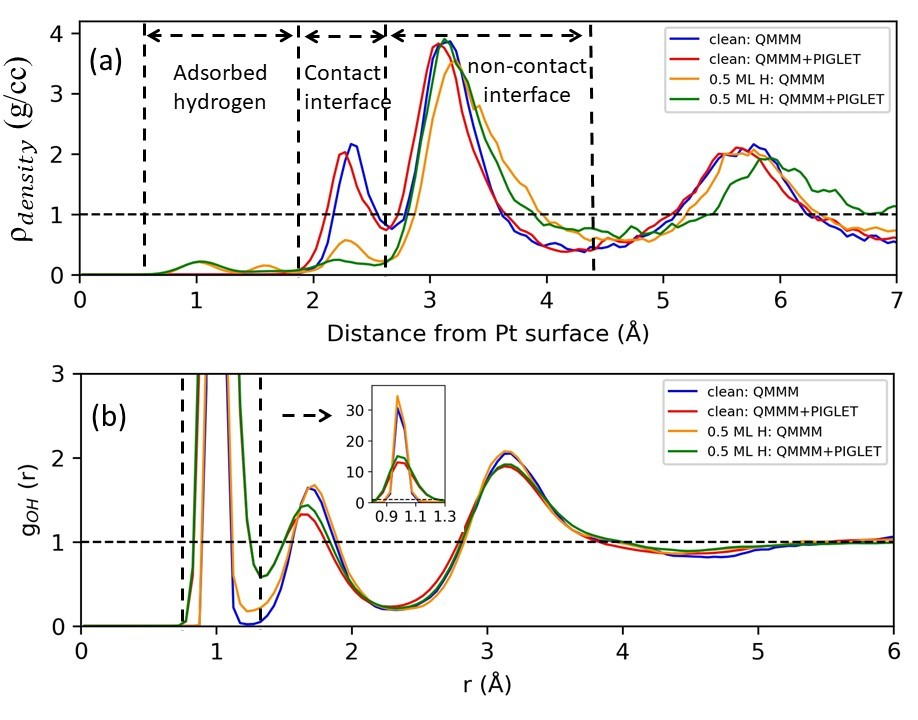
\includegraphics[width=15cm]{./Chapter3/figures/Slide1.JPG}       
   \end{center}
    \caption{(a) The planar average of water density (as per equation \ref{densitt}) as a function of its normal distance from the Pt surface for the clean and 0.5 ML H systems. (b) Radial distrbution function of O and H atoms at the interface (z $<$ 4.5 \AA{} from the surface) of the two systems. The first peak is magnified in the inset and corresponds to the O-H covalent bonds in the water layer. Blue and red (orange and green) graphs correspond to the QMMM and QMMM + PIGLET simulations of the clean (0.5 ML) system respectively.}
  \label{fig:Slide1}
\end{figure}

Figure~\ref{fig:Slide1}(a) shows the density profile for the two
interfaces as obtained from QMMM and QMMM $+$ PIGLET simulations. The graph 
for the Pt(111)/water interface obtained from QMMM simulation (blue line
in Figure~\ref{fig:Slide1}(a)) shows that there is a significant
enhancement of the density of water near the interface compared to that
of 1 g/cc known for bulk water. The density attains the bulk value
at distances beyond 7 \AA~from the surface. Moreover, close to the
surface we observe two peaks, a shorter one at about 2.32 \AA~apart from
the Pt(111) surface and a second longer one at about 3.18 \AA~away from 
the surface. Careful inspection of the QMMM trajectory for this interface
shows that the first peak is due to presence of chemisorbed water
species on the top of the surface Pt atoms (Figure~\ref{fig:Slide8}(a)). Based on the
density profile the water layers near the interface can be
divided into two distinct regions: (i) the interface region ($2.0 < z < 4.5$ \AA) that has a bilayer structure containing chemisorbed water molecules (contact interface) with Pt-O distance of 2.32 \AA{} and non-chemisorbed interacting water layer (non-contact) and (ii) transition region ($4.5<z<7.0$ \AA{}) in which
the water molecules are interacting with both the interface and bulk layer. 
We find that while in the contact (chemisorbed) interface region the water coverage is 0.18 ML, the total interface region has a coverage of 0.78 ML.

\begin{figure}
   \begin{center}
    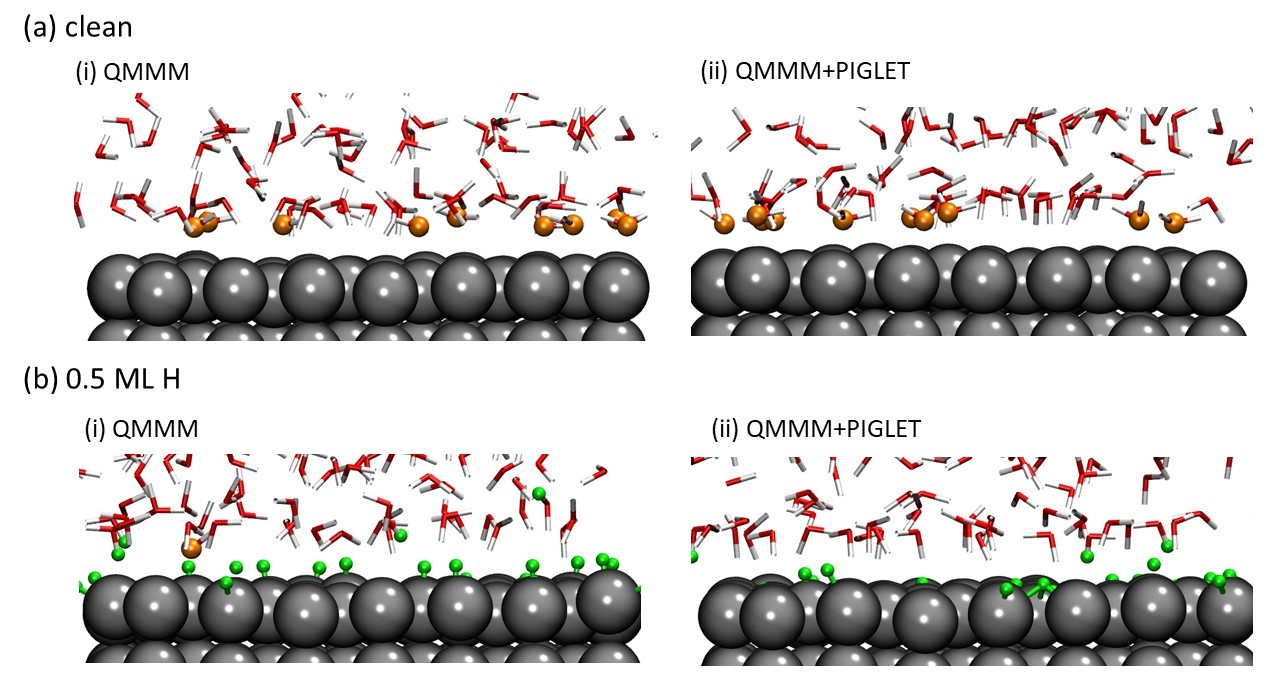
\includegraphics[width=15cm]{./Chapter3/figures/Slide8.JPG}       
   \end{center}
    \caption{Random snapshots of the (a) clean and (b) 0.5 ML H Pt(111)/water systems where (i) and (ii) correspond to the QMMM and QMMM $+$ PIGLET simulations respectively. The orange colour  balls refer to the chemisorbed oxygen atoms and the green colour balls are used to identify the adsorbed hydrogen atoms initially placed at the ``fcc" site. This colour code is followed in all the figures of this chapter. }
  \label{fig:Slide8}
\end{figure}

Upon turning on the NQE, we observe spontaneous splitting of water into
H and OH species with the OH being chemisorbed on the surface and the
H atom gets solvated primarily in the non-contact interface region (Figure~\ref{fig:Slide8}(b)). More details of the 
consequences of this splitting is described in the latter part of this
chapter. The planar average of the density computed from the equilibrated
QMMM $+$ PIGLET trajectory (red line in Figure~\ref{fig:Slide1}(a)) is similar
to that obtained from the QMMM trajectory with a slight overall shift towards
the surface suggesting a slight strengthening of the interaction
with the Pt surface. The position of the two peaks obtained from 
QMMM simulation at 2.32 and 3.18 \AA{} shifts closer to the 
surface at 2.28 and 3.08 \AA{} in the QMMM $+$ PIGLET simulation. Further,
we do not observe any significant change in the coverage of the water
layer on the Pt(111) surface. These suggest that though the quantum
fluctuations result in microscopic changes, these are not reflected
in the density, an overall macroscopic property.

These observations in the density profile described in the earlier
paragraphs are in reasonably good agreement with literature
reports\cite{lan2020ionization,gross2022ab}. For example, consistent with our results, Lan et al. obtained
values of 2.2 and 3.1 \AA{} for the first two peak positions
of the water density profile from their PIGLET simulations
at 298 K.\cite{lan2020ionization} Further, we note that the formation of the bilayer depends on the nature of the interactions between
metal and the water layers. Compared to the Pt(111) surface, the relatively less reactive Au(111) and Ag(111) surfaces\cite{le2018structure,li2021establishment} do not form bilayer and has a single peak around 2.6 \AA{} away from the surface whereas on Pd(111) surface\cite{le2018structure} the bilayer structure is preserved. In the special case of highly reactive Ru(0001) BOMD
simulations show that there is partial dissociation of interface water molecules into hydroxides and protons, resulting in only a single peak at around 2.2 \AA{} away from the surface.\cite{feibelman2002partial,maier2014unveiling}    

When the Pt surface is covered with 0.5 ML of H atoms
(Pt(111)-0.5 ML H/water interface) we observe significant changes
in its density profile (yellow and green plots in Figure \ref{fig:Slide1} (a) corresponding to QMMM and QMMM $+$ PIGLET respectively). The density profile can be demarcated into three regions namely chemisorbed hydrogen region ($z< 1.9$ \AA{}), the interface water region ($ 1.9 <= z < 4.5$ \AA)
and the transition water region ($4.5 < z < 7$) \AA{}.
The peak positions in the interface region are centered at 2.28 and 3.22 \AA{} in the QMMM simulation, which in the presence of NQEs move closer to the Pt surface at 2.22 and 3.08 \AA{}. This behaviour reaffirms that NQE strengthens the Pt-water interaction. Compared to the Pt(111)/water interface and irrespective of the NQEs, the chemisorption peak is significantly reduced in the semihydrogenated case. In case
of QMMM $+$ PIGLET simulations, the chemisorption peak is almost zero. This reduction in the chemisorption peak
can be attributed to the fact that the presence of H atoms
on the surface results in reduction of interaction between the
water molecules and the Pt surface.

Additionally, we also observe that NQEs pushes the transition region away from the surface. This behaviour is linked to the relatively shorter chemisorbed peak of the quantum nuclei simulation (with respect to the classical nuclei) where the desorbed molecules pushes some of the molecules into the transition region. Unlike the interface at the clean system, the H covered interface is dominated by a single dense peak that interacts with the surface Pt atoms. 

In order to understand the manifestations of the NQE on OH covalent bonds of
the water molecules and the H-bonds between the water molecules, we have
plotted the OH radial distribution function ($g_{OH}$) shown
in Figure~\ref{fig:Slide1}(b). The inset of Figure~\ref{fig:Slide1}(b)
shows the first peak corresponding to the covalent O-H bond. We
observe that the delocalization effect of the quantum nuclei results
in larger fluctuations of the O-H bond (1.00 \AA~for QMMM
and 1.02 \AA~for QMMM $+$ PIGLET) though the peak positions are similar (1.00 \AA~for QMMM
and 1.02 \AA~for QMMM $+$ PIGLET). The second peak in Figure~\ref{fig:Slide1}(b) corresponds to the inter-molecular H-bond lengths. In this case we observe that when NQE
is turned on, the peak position reduces from 1.75 to 1.70 \AA~suggesting
that the H-bonds are strengthened. We also observe significant broadening of the peak due to NQEs.


\subsubsection{Charged species in liquid water}

%Bulk water primarily consist of neutral water molecules and a small fraction of auto-dissociated hydroxide and hydronium ions owing to the small ionic product of water (10$^{-14}$ mol$^2$ L$^{-2}$)\cite{perlt2017predicting}. 
As described in the previous section, NQE results in transient 
dissociation of the water molecules at the Pt(111)/water interface
that results in protons released in water and the OH species
bound to the surface. Moreover, it is also known that NQE results in
auto-dissociation of bulk water at high temperature and pressure \cite{ceriotti2016nuclear}. Further, when the surface is 
hydrogenated, i.e. Pt(111)-0.5 ML H/water, we observed that there is 
desorption of protons from the surface into the bulk water. These processes results in the formation
of charged species at the water interface. In this section we will discuss
the different types of species that are formed and how their concentration
varies as one moves away from the surface.

The various species in water can be identified by counting the number of covalent O-H bonds an oxygen atom possesses, i.e. through the coordination number of oxygen atoms ($CN_{O}$). We have used the recipe proposed by Hassanali et al.\cite{hassanali2011recombination}, which provides a continuous value to quantify the number of O-H covalent bonds and
can be expressed as:

\begin{align}
\label{cno}
CN_{O} = \sum_{J=1}^{N_H} \frac{1-(\frac{|R-R_J|}{r_o})^{16}} {1-(\frac{|R-R_J|}{r_o})^{56}} \hspace{1cm}  
\end{align}

\noindent where, $N_H$ is the number of H atoms in the system, $J$ is the index of the H atom and  $R$ and $R_J$ are the positions of O and the $J^{th}$ H in the system,
respectively. The cutoff value, $r_o$, of 1.32 \AA{} is the limit of covalency for the O-H bond. The $CN_{O}$ values of 0, 1, 2 and 3 represent oxide ion, hydroxide ion, water molecule and hydronium/Eigen/Zundel ions respectively. 

\begin{figure}
   \begin{center}
    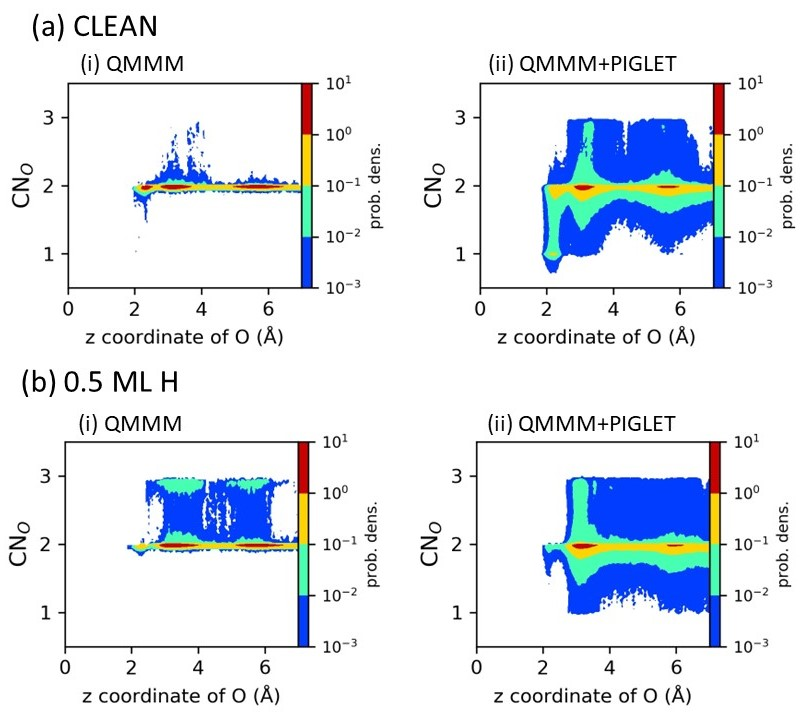
\includegraphics[width=15cm]{./Chapter3/figures/Slide2.JPG}       
   \end{center}
    \caption{Joint distribution of the coordination number of oxygen ($CN_{O}$, as per equation \ref{cno}) with its normal distance from the Pt surface for the (a) clean and (b) 0.5 ML H systems. (i) and (ii) correspond to the respective QMMM and QMMM $+$ PIGLET simulations of either systems.}
  \label{fig:Slide2}
\end{figure}

The presence of ions in the water layer is ascertained by plotting the 
joint probability distribution between $CN_O$ and the normal distance
of the O atom from the surface Pt atoms (Figure \ref{fig:Slide2}). The coordination value of oxygen atoms in the QMMM 
simulation (Figure \ref{fig:Slide2} (a-i)) of the Pt(111)/water system  
is primarily $\sim$ 2 with small fluctuations in the interface region. 
Thus, the liquid layer is ion free and contains neutral water molecules. 
A careful inspection of the configurations corresponding to those small 
deviations show an elongation of the O-H along their hydrogen bonds (O-H$\cdots$O) at the contact interface layer. 
%The first peak of the O-H pair correlation (g$_{OH}$, Figure \ref{fig:Slide1} (b)) of the interface water molecules (z $<$ 4.5 \AA{}) represent the O-H covalent bond with a mean (standard deviation) value of 1.00 (0.004) \AA{}. The formation of the less dense contact layer is due to the chemisorption of the water molecules where the oxygen of water binds on the top site of the surface Pt atom. A snapshot of the chemisorbed water molecules (shown as green balls) on the Pt surface is shown in Figure \ref{fig:Slide8} (a-i). The chemisorbed water molecules do not perennially localise on the surface and undergo continuous exchange from the non-contact layer. The average coverage of the oxygen atoms in the contact layer is 0.17  which suggests that only a small fraction of Pt atoms form chemical bonds with water molecules. On the other hand, the non-contact layer contains water molecules which at one end interacts with the surface Pt and chemisorbed water molecules and on the other end interacts with the water molecules in the transition region. The coverage of the oxygen atom in this region is 0.60 in accordance with its higher density. 

The incorporation of NQE (via QMMM $+$ PIGLET) causes quantum fluctuations in the O-H covalent bonds of the water molecules. 
%These fluctuations originate from the zero point motion of the bonds. As a result, the standard deviation in the O-H covalent bond distances for the interface molecules increases to 0.02 \AA{} with an unchanged mean value of 1.02 \AA{}. 
These result in dissociation of about 16\% ($\frac {freq (chemisorbed\, hydroxyl)}{freq (chemisorbed\, water)} * 100$) of the chemisorbed water molecules into hydroxide species (bound to the surface) and solvated protons. The hydroxide binds on the top site of the Pt surface which is evident from the large probability density with $CN_{O} = 1$ at 2.32 \AA{} from the Pt surface (Figure \ref{fig:Slide2}(a-ii)). Further, the smaller proportion of oxygen atoms with $CN_{O}$ around 1 away from the contact layer are related to the solvation of the proton and are discussed below in detail. 

The proton from the chemisorbed water molecule is abstracted by the water molecule in the non-contact layer which in turn forms a chain like network of the solvated proton as shown in Figure \ref{fig:Slide9}(i-a). This structure has a transient life and breaks down into a Zundel cation (Figure \ref{fig:Slide9}(i-b)) where two water molecules share the excess proton. As a consequence the $CN_O$ value of the participating oxygen atoms increases to more than 2.5. With the evolution in simulation
time, the shared proton moves closer to one of the two participating oxygen atoms whereas a different hydrogen attached to the oxygen gets shared with a neighbouring water molecule. As a result, the oxygen atom momentarily has one covalently bonded proton with the other two being shared. This is reflected in the lowering of the $CN_O$ away from the chemisorbed interface layer as mentioned in the previous paragraph. The complete process leads to the propagation of the Zundel cation in the solution. Figure \ref{fig:Slide2}(a-ii) shows the $CN_O$ value close to 3, which represents the solvated proton. We note that this is not confined to the interface region and extends deep inside the solution with a reduced probability density suggesting that even away from the surface protonation and deprotonation events are occurring, though their probability is less. Sometimes, the thermal fluctuations momentarily break the propagation of Zundel cation by dissociating into hydronium ion (Figure \ref{fig:Slide9}(i-c)) and water molecule. In very rare and transient cases, this hydronium could form hydrogen bonds with three neighbouring water molecules to generate the Eigen cation (Figure \ref{fig:Slide9}(ii-b)). Overall, the three ionic species namely hydronium, Eigen and Zundel are ideal structures which have transient existence\cite{marx1999nature} and are forms of the solvated proton. However, the uniform distribution of $CN_O$ plot (Figure \ref{fig:Slide2}(a-ii)) between three and two in the solution suggest that the Zundel cation and its chain like forms are preferred. We note that this has also been recently detected by experiments\cite{tian2022visualizing}.  

\begin{figure}
   \begin{center}
    \includegraphics[width=15cm]{./Chapter3/figures/slide9.JPG}       
   \end{center}
    \caption{Random snapshots of the clean system obtained from the QMMM $+$ PIGLET simulation showing (i) the solvated proton in different forms (blue balls): (a) chain-like ion, (b) Zundel ion and (c) hydronium ion. Additional snapshots to illustrate (ii) the recombination of hydroxide from (a) solvated proton and (b) chemisorbed water indirectly (left panel) and directly (right panel).}
  \label{fig:Slide9}
\end{figure}

Lan et al.\cite{lan2020ionization} reports the solvated proton recombines with the adsorbed hydroxide to give back the chemisorbed water molecule. In agreement, we also find the recombination of the solvated proton shown in Figure \ref{fig:Slide9} (ii-a). However, the recombination of hydroxide with the solvated proton is not the only recombination process. Additionally, the adsorbed hydroxide can be converted to water molecule through two distinct re-combinations that do not involve the solvated proton. In one scenario, shown in Figure \ref{fig:Slide9} (ii-b:indirect), a neutral water molecule in the non-contact layer (blue) abstracts one of the hydrogen atom from a nearby chemisorbed water and donates it to the hydroxide. The process is concerted and causes the oxygen of the non-contact water molecule to have an incoming and outgoing proton. These events also increase the proportion of $CN_{O} = 3$ at the non-contact layer. The other recombination process is achieved by the direct transfer of proton from a proximal chemisorbed water molecule as shown in Figure \ref{fig:Slide9} (ii-b:direct). In the last two recombination processes, the number of hydroxide species on the surface is preserved.  

The dissociation and recombination events can be represented by the following equilibrium:
\begin{equation}
    Pt-H_2O + nH_2O (aq) \rightleftharpoons Pt-OH^- + H^+(H_2O)_n(aq)  
\end{equation}
Since the dissociated protons from the chemisorbed water are solvated while the hydroxide ions do not, the overall aqueous layer becomes acidic. The acidity of the solution is quantified by the pH which is calculated in the following way. 

\begin{equation}
    pH=-ln(\frac{number\, of\, moles\, of\, solvated\, proton}{Volume\, of\, solution})
\end{equation}

\noindent As described in the last paragraph, the solvated proton $H^+(H_2O)_n(aq)$ exists in multiple forms which makes it challenging to identify and quantify them accurately. Additionally, the auto-dissociation of aqueous water into hydroxide and proton increases the complexity in quantifying the number of moles of solvated proton. For the sake of simplicity, the number of protons from auto-dissociation events have not been included in the calculation of the pH and  only the protons generated from the dissociation of the chemisorbed water are counted. The latter is indirectly estimated from the number of bound hydroxides which are quantified by the $CN_O$ value of less than 1.5. 
%Further, since the MM water cannot dissociate due to the use of non-polarisable (SPCE-modified) forcefield, the volume of the water solution is also restricted to the QM region. 
Therefore in this present context, the pH of the interface solution is calculated using the following equation.

\begin{equation}
    pH=-ln(\frac{number\, of\, moles\, of\, bound\, hydroxide}{Volume\, of\, QM\, water\, solution})
\end{equation}

With all these restrictions, we estimate the pH of the water layer at 1.42. The acidic nature of the interfacial water is also reported experimentally\cite{rizo2015towards,martinez2015exploring}.


Similar to the Pt(111)/water interface, in the Pt(111)-0.5 ML H/water
interface we also observe different charged species. Here, the charged
species are observed in both the QMMM and QMMM $+$ PIGLET trajectories due
to transfer of the absorbed H atoms from the Pt surface into water. The joint probability distribution of the coordination number of the oxygen atoms with their positions relative to the Pt surface along the normal is shown in Figure \ref{fig:Slide2}(b). The plots for both the simulations (QMMM: Figure \ref{fig:Slide2}(b-i) and QMMM $+$ PIGLET : Figure \ref{fig:Slide2}(b-ii)) has a $CN_O$ value of 3 in the water region which confirms that the extra hydrogen atoms entering the water layer are solvated protons. Here also the solvated protons are highly mobile and propagate in the water layer through the help of the Zundel cation and its chain structure. Figure \ref{fig:Slide10}(b,c and d) contains representative snapshots of the different forms of solvated proton. A closer inspection reveals all the hydrogen atoms are abstracted from its less stable ``top" site on the Pt surface and is shown in Figure \ref{fig:Slide10}(a). 

\begin{figure}
   \begin{center}
    \includegraphics[width=15cm]{./Chapter3/figures/slide10.JPG}       
   \end{center}
    \caption{Random snapshots of the 0.5 ML H system obtained from either QMMM or QMMM $+$ PIGLET simulation showing the (a) abstraction of adsorbed hydrogen atom  and the solvation of proton in three different forms (blue balls): (b) chain-like ion, (c) Zundel ion and (d) hydronium ion. Orange coloured balls show the chemisorbed water molecules/hydroxide ions. }
  \label{fig:Slide10}
\end{figure}

During the course of our sampling period, we find 14 \% of initially adsorbed hydrogen atoms gets solvated at the end of either simulation. This decreases the pH to 0.52 and makes the water layer acidic. Similar to the clean case, the volume of the solution used to calculate the pH is restricted to the QM region. The desorption of adsorbed hydrogen into the water layer leads to the oxidation (reduction) of the hydrogen (platinum) and is expressed by the Volmer reaction:       

\begin{equation}
    \label{}
    Pt-H + nH_2O (aq) \rightleftharpoons Pt ^- + H^+(H_2O)_n (aq)
\end{equation}

%The corresponding equilibrium constant is given by:
%\begin{equation}
%    K_{eq}^{H} = \frac {[H_3O^+]} {[H_2O]}
%\end{equation}
%where, the terms in the square brackets are the concentrations of hydronium ion ($[H_3O^+]$) and water ($[H_2O]$). The $pK_{eq}^{H_2O}$ value for the desorption of adsorbed hydrogen is ...  


%Unlike the clean system, NQEs do not bring about any drastic change in the liquid layer but a significant manifestation is observed for the adsorbed hydrogen atoms. In the next section, we report the electrochemistry of the hydrogen covered ``0.5 ML" Pt/water system. 

%The dissociation reaction and the corresponding equilibrium constant are written below:  
%\begin{equation}
%    \label{}
%    Pt-H_2O + nH_20 (aq) \rightleftharpoons Pt-OH^- + H+(H_2O)_n(aq)  
%\end{equation}
%The corresponding equilibrium constant is given by:
%\begin{equation}
%    K_{eq}^{H_2O} = \frac {[Pt-OH^-][H^+(H_2O)_n]} {[Pt-H_2O]}
%\end{equation}
%where, the terms in the square brackets are the concentrations of the respective species ($Pt-OH$, $H_3O^+$ and $H_2O$). Since the dissociated entities originate from the chemisorbed water, we assume the concentration of hydroxyl ($[Pt-OH]$) and solvated proton ($[H_3O^+]$) to be same and is calculated from the number of O-H inside the contact layer. The $pK_{eq}^{H_2O}$ value for the dissociation process is 11.23 which is much lower than the value of 6.04 reported by Lan et al.\cite{lan2020ionization} from their \textit{ab  initio} PIGLET simulation.  

Overall, we find that the quantum nuclei simulation (QMMM $+$ PIGLET) is able to capture the dissociation events that are not accessible through the classical nuclei simulation (QMMM). Although the microscopic structure of interface is a structural property, it affects the electrochemical property by altering the work function of the metal. Therefore, in the next section, we discuss the interfacial properties affecting the work function of the water covered metal electrode in the presence and absence of NQEs. 

\subsubsection{Electrochemical property at the interface}

The electrochemistry of the interface is governed by the electrode potential of the electrchemical cell. Trasatti et al.\cite{trasatti1983structuring} showed that the electrode potential is related to the work function of the water covered metal which is sensitive to (i) the electronic rearrangement due to the interaction between the electrode and the solvent and (ii) the preferential orientation of the polar solvent molecules. Hence, to understand the role of NQEs on the electrochemical properties of the interface, we have computed the work function change ($\Delta$WF) in the Pt electrode due to the creation of interfacial dipole from (a) the charge reorganization between solvent and electrode ($\Delta$WF$_{ele}$) and (b) the preferential orientation of the water species in the presence of the electrode ($\Delta WF_{ori}$).

%relation between the absolute electrode potential and the work function of water covered metal surface. With respect to our present slab model, the work function of the water covered metal surface (WF$_{metal-water}$) is evaluated as the difference in the Fermi level of the Pt/water system and the vacuum level obtained from the constant electrostatic energy on top of the liquid layer. On the other hand, the work function of the metal/vacuum interface is the difference in the Fermi level of the Pt/water system and the vacuum level on the other side of the slab where water layer is absent\cite{hansen2016ph}. Thus, the presence of the water film leads to the change in work function ($\Delta$ WF = WF$_{metal-water}$ - WF$_{metal-vac}$). This alteration of the work function is related to the interface processes like adsorption, charge reorganization, orientation of polar bonds and the presence of ions. The total change ($\Delta WF$) is broadly categorised into electronic ($\Delta$ WF$_{ele}$) and orientational ($\Delta$ WF$_{ori}$) contributions, where the former constitutes of dipole generation due to charge reorganization (adsorption, polarisation and ion formation) and the latter addresses the dipole formation due to orientation of the polar O-H bonds.  

%In the case of ion-free water, the electrode potential is termed as the potential of zero charge (PZC $=\frac{WF_{metal-water}}{e}$. %The PZC is one half of a cell reaction is usually reported with respect to the standard hydrogen electrode (SHE) electrode (PZC vs SHE) where potential for the SHE half reaction is equal to 4.44 V.  

\subsubsection*{Electronic contribution to the change in work function}
\label{wf_ele}
The electronic contribution to the change in work function is related to the reorganization of the charge density when the water layer interacts with the metal atoms. For the QMMM/QMMM $+$ PIGLET simulations, this reorganization ($\Delta\rho$) is computed as:

\begin{equation}
\Delta\rho(r) = \rho (r)[metal+ solvent] - \rho (r)[metal] - \rho (r)[solvent]
\label{delrho}
\end{equation}

\noindent where, $\rho (r)[metal+solvent]$ is the charge density of
the full system, i.e., all the Pt atoms, H atoms where applicable, and 
the water molecules
included in the QM region. $\rho (r)[metal]$ is the charge density of
the Pt atoms representing the electrode. $\rho (r)[solvent]$ is the 
charge density of the water molecules in the QM region. 
For Pt(111)-0.5 ML/water, the charge density due to H atoms are also included in $\rho [solvent]$. Moreover, while computing
the second and third terms on the right hand side of Eqn.~\ref{delrho}
the individual components are kept in
the same geometry as that in the combined system.

The plots of the charge density difference isosurfaces for a random snapshot
from the Pt(111)/water and Pt(111)-0.5 ML H/water trajectories are shown 
in Figure~\ref{fig:Slide11} (a) and (b) respectively. The blue (yellow)
isosurface shows charge depletion (accumulation). It is evident that the 
charge reorganization is restricted to the surface Pt atoms and the 
interface (z $<$ 4.5 \AA{}) water molecules. Further, for the Pt(111)
interface, only the water molecules with a H-down configuration (where 
one hydrogen atom points towards the surface and the other is nearly 
parallel to the surface) and the chemisorbed ones contribute towards
charge transfer. When the surface is covered with 0.5 ML of H, only the water molecules with H-down configurations contribute to the charge transfer process (Figure~\ref{fig:Slide11}(b)). This is in accordance with the fact that the chemisorbed H atoms reduces the interaction between the Pt electrode and water thereby desorbing almost all the chemisorbed water molecules. Further, the charge reorganization finds the chemisorbed H atoms to accumulate the majority of the charge density. 

%Interestingly, as mentioned in the previous section, the incorporation of
%NQEs makes the water layer acidic due to the transient splitting
%of the interfacial water molecules. 
%As a result, the system of solvated water layer contains a finite
%concentration of positively charged hydronium ions and is not ion free as widely reported\cite{sakong2018electric,le2017determining} using simulations where the nuclei are treated classically. We note that the  formation of solvated ions in the water layer introduces the complexity of treating the charged cation species in the water fragment and needs a more rigorous representation. Nonetheless, in this chapter, we report the analysis and the values for comparison. 

The charge reorganization is quantified by computing the
time averaged planar average of the charge density difference 
($\Delta\rho (z)$) along the surface normal. For each of the plots 100
random snapshots have been selected to compute the time average. Figure~\ref{fig:Slide5} (a/b-i) shows the plots for
$\Delta\rho (z)$. A negative (positive) value corresponds to charge 
depletion (accumulation). The scale along the z-axis is adjusted such 
that the origin of the z-axis is at the average position of surface Pt atoms that
are in contact with water/H atoms. 
For the Pt(111)/water interface (Figure~\ref{fig:Slide5} (a-i)) we observe a charge accumulation region between the electrode surface and the water layer interacting with 
the Pt atoms (0 $<$ z $<$ 2 \AA{}). Complementary to the charge accumulation region, a charge depletion region is observed in the interfacial water layer (2 $<$ z $<$ 4.5 \AA). This results in creation of a surface dipole along the surface normal pointing away from the surface. The potential generated by the dipole reduces the barrier for electron abstraction from the metal electrode.  

The situation is more complex in the Pt(111)-0.5 ML H/water interface. We observe two regions of charge accumulation and depletion, namely, between the Pt atoms and the H (0 $<$ z $<$ 0.58 \AA{}) and a second one starting from the adsorbed H atoms and extending to the interfacial water layer (0.58 $<$ z $<$ 4.5 \AA{}). The magnitude of dipole generated due to water reorganization (0.58 $<$ z $<$ 4.5 \AA{}) is larger than the dipole generated due to the interaction of hydrogen with surface Pt atoms (0 $<$ z $<$ 0.58 \AA{}). This double dipole at the H covered interface is relatively less effective in extracting the electrons when compared to the clean surface where a single large dipole is witnessed. 

%The charge accumulation region constitutes of two peaks generated due to the contributions from two kinds/types of water molecules. The individual contributions ($\Delta\rho_{1,2}$) are calculated using the following equations: 
%\begin{equation}
%\Delta\rho_1 = \rho [metal + water] - \rho [metal + ads.\,species] - \rho [water - ads. \,species]
%\end{equation}
%\begin{equation}
%\Delta\rho_2 = \Delta\rho - \Delta\rho_1 
%\end{equation}

%where $\rho [metal + ads.\,species]$ and $\rho [water - ads.\,species]$ is the charge density of fragment system consisting of metal with adsorbed species (only water molecules in the case of clean QMMM) and water layer without the adsorbed species. Figure \ref{fig:Slide4} in the Appendix \ref{appendix5} shows the first depletion peak closer to the surface comes from adsorbed layer water molecules ($\Delta\rho_1$, blue dashed curve) whereas the second peak farther away from the surface comes from the non-adsorbed water layer ($\Delta\rho_2$: blue solid line). It is interesting to note that the fluctuations in the charge difference within the metal slab is primarily due to the adsorbed/chemisorbed species. 

%Integration of the charge difference graph ($\Delta\rho$) in the water region show a depletion of 1.68 electrons from the complete water layer which is jointly shared by the surface Pt atoms. This generates a dipole moment ($\mu_{ele}$) from the negatively charged Pt surface towards the water. The potential due to this charge induced dipole lowers the work function of the Pt metal in the Pt/water system. 
%This ion free water layer obtained from the QMMM simulation corresponds to the potential of zero charge (PZC) of the metal/water interface.

The change in the work function due to charge redistribution at the
interface ($\Delta$WF$_{ele}$) is given as:\cite{chen2022modeling}

\begin{equation}
    \label{wf_elee}
    \Delta \textrm{WF}_{ele}  = -\frac{e}{(l_xl_y)\epsilon_0 }\int_{metal}^{vacuum} z  \Delta\rho (z)  dz
\end{equation}

\noindent where, $e$ and $\epsilon_0$ are the values of a unit charge and
permittivity of vacuum, respectively. $l_xl_y$ is the area of the Pt surface. The limits of the integration 
extends throughout the simulation cell. The probability distributions
of $\Delta$ WF$_{ele}$ for Pt(111)/water at T=298 K, with and without NQE 
are shown in Figure \ref{fig:Slide5}(a-ii). Without incorporating
the NQE, the average value of $\Delta$ WF$_{ele}$ is estimated to
be -1.64 eV ($\pm$ 0.12 eV). 
This shows that the surface dipoles created at the interface, which
is a consequence of charge redistribution due to the interaction
between the Pt electrode and the water layer, indeed eases the electron abstraction by -1.64 eV. Upon turning on the NQEs, the work function is further reduced by about 0.08 eV. Similarly, Litman et al.\cite{litman2018decisive} finds that NQEs decrease the work function change by 0.04 eV for Pt(221)/water interface by increasing the dissociation probability of chemisorbed water.

For the Pt(111)-0.5 ML H/water interface, we obtain an average reduction
in the work function at -1.46 eV ($\pm$ 0.14 eV). We note that compared to the
Pt(111)/water interface, here the magnitude of work function change
is less, which is in accordance with the charge transfer plot where we
observed a double surface dipole. Moreover, in this case, upon incorporating
the NQE, the work function is reduced further by about 0.22 eV.
Our results show that the nuclear quantum fluctuations affect the
electronic properties more strongly when the surface is covered
with H atoms.

%Thus, the change in work function (Figure \ref{fig:Slide5}(a-ii)) due to the electronic rearrangement is estimated at -1.64 ($\pm$ 0.12) eV which slightly overestimates the values obtained by other reports\cite{li2021establishment,le2017determining}. 


\begin{figure}
   \begin{center}
    \includegraphics[width=15cm]{./Chapter3/figures/slide11.JPG}       
   \end{center}
    \caption{Random snapshots showing the charge reorganization (between the slab and the combined system of water and any chemisorbed H for the (a) clean and (b) 0.5 ML H systems obtained from (i) QMMM and (ii) QMMM $+$ PIGLET simulations. The iso value of the iso-surface is 0.01 e/bohr$^3$. Blue (yellow) isosurface corresponds to charge depletion (accumulation).}
  \label{fig:Slide11}
\end{figure}

\begin{figure}
   \begin{center}
    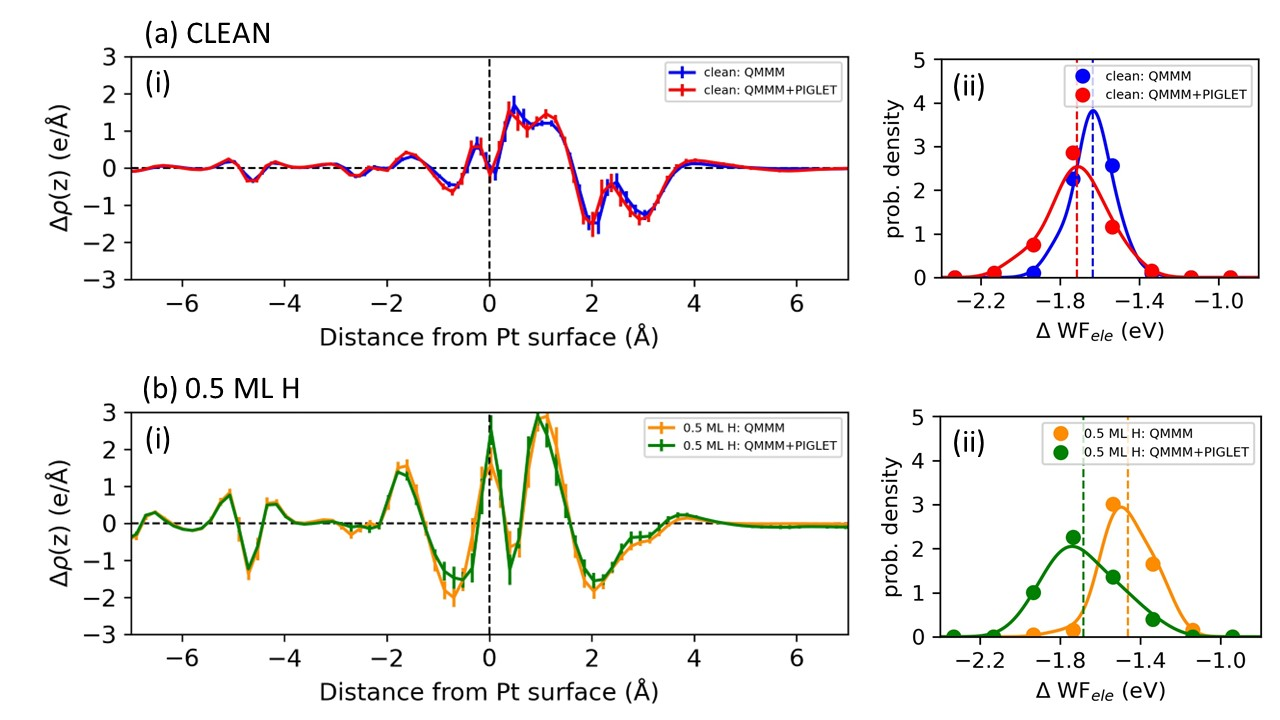
\includegraphics[width=16cm]{./Chapter3/figures/Slide5.JPG}       
   \end{center}
    \caption{(i) The charge density difference ($\Delta\rho$) along the surface normal and (ii) the corresponding change in work function for the (a) clean and (b) 0.5 ML H systems obtained from 100 random snapshots. Blue and red (orange and green) graphs correspond to the QMMM and QMMM + PIGLET simulations of the clean (0.5 ML) system respectively.}
  \label{fig:Slide5}
\end{figure}

\subsubsection*{O-H bond orientational dipole contribution to the change in work function}
In addition to the electronic contribution to the modification in the work function of the Pt electrode, the net orientation of all the polar O-H covalent bonds along the surface normal also influences the work function\cite{gross2022ab}. Due to the
homogeneity in the bulk region, the O-H dipole moment cancels each other. However,
the interface is inhomogeneous, with a larger number of O-H bonds pointing
towards the surface due to interaction with the electrode. This results in finite
dipole moment that points towards the surface, thereby opposing electron removal
from the electrode.
  
The relative orientation of the covalent O-H bond with respect to the surface is represented through the angle $\theta$, the angle O-H vector makes with the surface normal and is schematically shown in Figure \ref{fig:Slide3} (a). A value of 0$^{\circ}$ (180$^{\circ}$) degrees implies that the O-H bond is parallel (anti-parallel) to the surface normal pointing away (towards) from the surface whereas a value of 90$^{\circ}$ implies that the O-H bond is parallel to the surface. In case of Pt(111)/water interface, the joint probability distribution plot of $\theta$ with the $z$ position of the oxygen atoms of the O-H bond for the chemisorbed water species peaks at around 50-90$^{\circ}$ (Figure \ref{fig:Slide3} (b-i/ii)) implying that the O-H bonds are almost parallel to the surface. However, the non-contact water layer has a bimodal distribution of the O-H bonds with peaks around 60-110$^{\circ}$ and 130-180$^{\circ}$. This suggests that there is a net orientation of O-H pointing towards the surface. The presence of hydrogen in the Pt(111)-0.5 ML H/water interface leads to water desorption which significantly reduces the proportion of O-H bonds in range of 50-90$^{\circ}$ as shown in Figure \ref{fig:Slide3} (c-i/ii). Compared to the clean system, this increases the relative proportion of configurations where the O-H bond points toward the surface. Overall, the clean and the 0.5 ML H systems with and without NQEs show a preferential orientation of the O-H covalent bond at the interface. 

\begin{figure}
   \begin{center}
    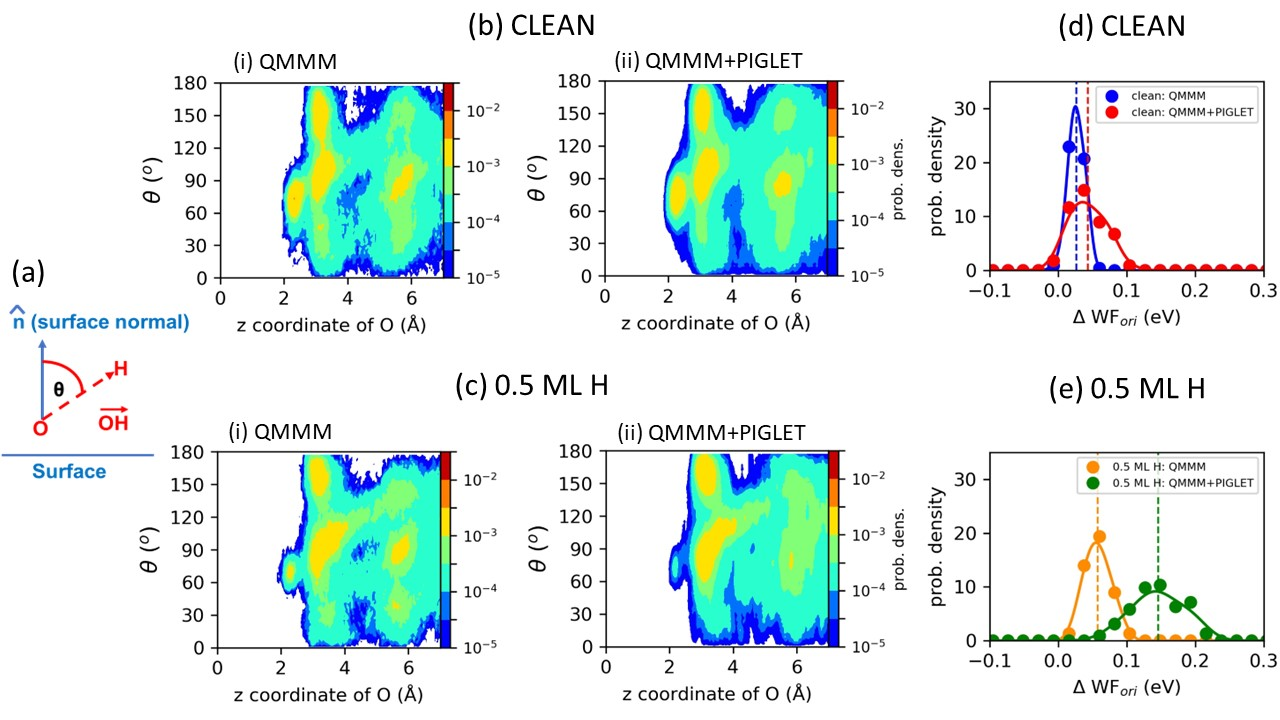
\includegraphics[width=15cm]{./Chapter3/figures/Slide3.JPG}       
   \end{center}
    \caption{(a) Schematic showing the definition of $\theta$ to quantify the orientation of the O-H covalent bond ($CN_O$ $<$ 1.5). The joint distribution of $\theta$ (in degrees) with its distance from the Pt surface along the surface normal for the (b) clean and (c) 0.5 ML H systems obtained from the (i) QMMM and (ii) QMMM $+$ PIGLET simulations. The corresponding work function change due to the preferential orientation of the polar O-H bond ($\Delta$ WF$_{ori}$) along the surface normal for the (d) clean and (e) 0.5 ML H systems obtained from the 100 random snapshots.}
  \label{fig:Slide3}
\end{figure}

Quantitatively, the work function change ($\Delta \textrm{WF}_{ori}$) due to O-H orientation is calculated using the following equation\cite{li2021establishment}:
\begin{equation}
    \label{wf_ori}
    \Delta \textrm{WF}_{ori}  =  -\frac{e}{(l_xl_y)\epsilon_o } <\mu_{OH}\, cos \,\theta_{res}>
\end{equation}

\noindent where, $\mu_{OH}$ is the dipole moment of the O-H covalent bond in water which has a value of 1.5 D\cite{tuckerman1997quantum}. $l_xl_y$ is the area of the Pt surface. $<\mu_{OH}\, cos \,\theta_{res}>$ is the ensemble average of the dipole moments along the surface normal for all the O-H covalent bonds.
%Thus, only the perpendicular component (0/180$^{\circ}$) of the O-H bond dipole interacts with the work function of the metal/water system. 
It it to be noted that in this approach we have assumed that the dipole moment
of the O-H bond is constant, irrespective of the change in the bond length
and the chemical environment.

The probability distributions of $\Delta$WF$_{ori}$ using the same 100 (random) snapshots used during the calculation of charge reorganization is shown in Figure \ref{fig:Slide3}(d) and (e) for Pt(111)/water and Pt(111)-0.5 ML H/water, respectively. In accordance with the qualitative assessment of a net O-H orientation towards the surface, the average values of $\Delta$WF$_{ori}$ for all the cases have a positive value. This suggests that the orientational dipole increases the work function making it harder to abstract electrons from the metal surface. However, this increase in work function is negligible with respect to the change introduced due to the electronic reorganization which has also been previously reported\cite{le2017determining,li2021establishment,sakong2018electric}. In the case of clean Pt(111)-water system, $\Delta$WF$_{ori}$ with and without NQEs is 0.03 and 0.04 eV which is smaller than that observed for the 0.5 ML H counterpart with values of 0.06 and 0.14 respectively. The results are in accordance with the fact that the presence of hydrogen increases the proportion of configurations where O-H points towards the surface. Overall, the NQEs seem to enhance the O-H down configurations. Similar to that observed for the electronic case, the NQEs are more pronounced when the surface is covered with H.

Combining the effects of charge redistribution and O-H dipole, the net work function changes ($\Delta$WF) for Pt(111)/water interface with and without NQEs are -1.61 and -1.67 eV respectively. In the presence of H atoms on the surface, i.e., Pt(111)-0.5 ML H/water the corresponding values increases to -1.41 and -1.54 eV respectively. Thus, our results show that NQEs facilitate the electron transfer process.


\subsection{Summary and Conclusions}
In summary, using our novel implementation we have integrated the inexpensive QMMM electronic structure method with the PIGLET simulations to investigate the structural and electrochemical properties of the clean and hydrogen-covered Pt(111)/water interface at room temperature. Our results show NQEs not only strengthens the water hydrogen bonds but also enhances the Pt-water interaction. In the case of the clean interface, the quantum delocalization of the O-H bond tends to dissociate some of the water molecules chemisorbed on the Pt(111) interface. The dissociated hydroxide stays bound to the Pt surface whereas the dissociated proton gets solvated into the liquid layer thereby making the water layer acidic. These solvated protons propagate throughout the water layer in a predominantly Zundel structure. 

On the Pt(111)-0.5 ML H/water interface, chemisorbed H at the Pt surface prevents the chemisorption of water molecules along with any dissociation activity. With or without NQEs, some of these chemisorbed H atoms desorb and solvate into the liquid layer. Similar to the clean system, the propagation of the solvated protons is dominated by Zundel structures. The quantification of the acidity reveals that the water layer over the H covered Pt(111) surface has a higher acidity compared to the clean interface. The interfacial structure at the metal electrode creates an interfacial dipole that modifies the electrode potential by altering the work function of the metal. The interfacial dipole is composed of two individual dipoles: one generated by charge reorganisation and the other by preferential orientation of the O-H polar bonds. The charge induced dipole reduces the work function of the metal while the orientational dipole enhances it. However, the latter is much smaller in magnitude compared to the former. In the presence of chemisorbed H, the work function is reduced due to the interaction of the hydrogen with the Pt surface. Overall, the presence of water layers reduce the work function of the Pt electrode which are enhanced by NQEs.